% -----------------------------------------------
% Vlastní text práce (kapitoly práce)
% -----------------------------------------------

% -----------------------------------------------
\chapter{FAST telescope}
% -----------------------------------------------
The  Fluorescence  detector  Array  of  Single-pixel  Telescopes  (FAST) is an international R$\&$D project of fluorescence telescopes sensitive to UHECRs. 
\par
As of today there are four prototypes in active service. Three of them are situated in Black Rock Mesa site of the Telescope Array experiment in central Utah and one in Argentina within Pierre Auger Observatory.
\par
The main goal of FAST project is to develop a cheap fluorescence telescope, which could be used in future to cover a wide surface area. This new oncoming fluorescence telescope array should be able  
to fully reconstruct the geometry of UHECRs induced UV shower by combining the information from multiple telescopes.

\begin{figure}[H]
 \centering
    \subfloat[][\centering Telescope design \cite{MALACARI2020102430}.]{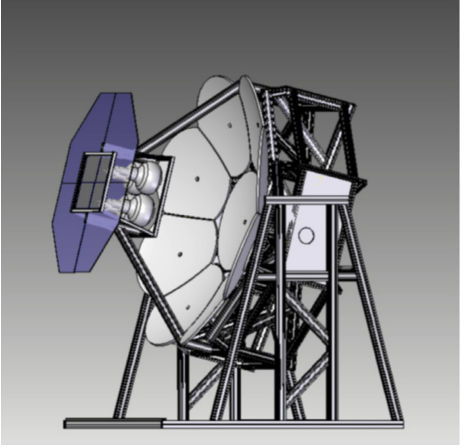
\includegraphics[scale = 0.48]{./pictures/fastTheoretical}}%
    \qquad
    \subfloat[][\centering Prototype \cite{Project}.]{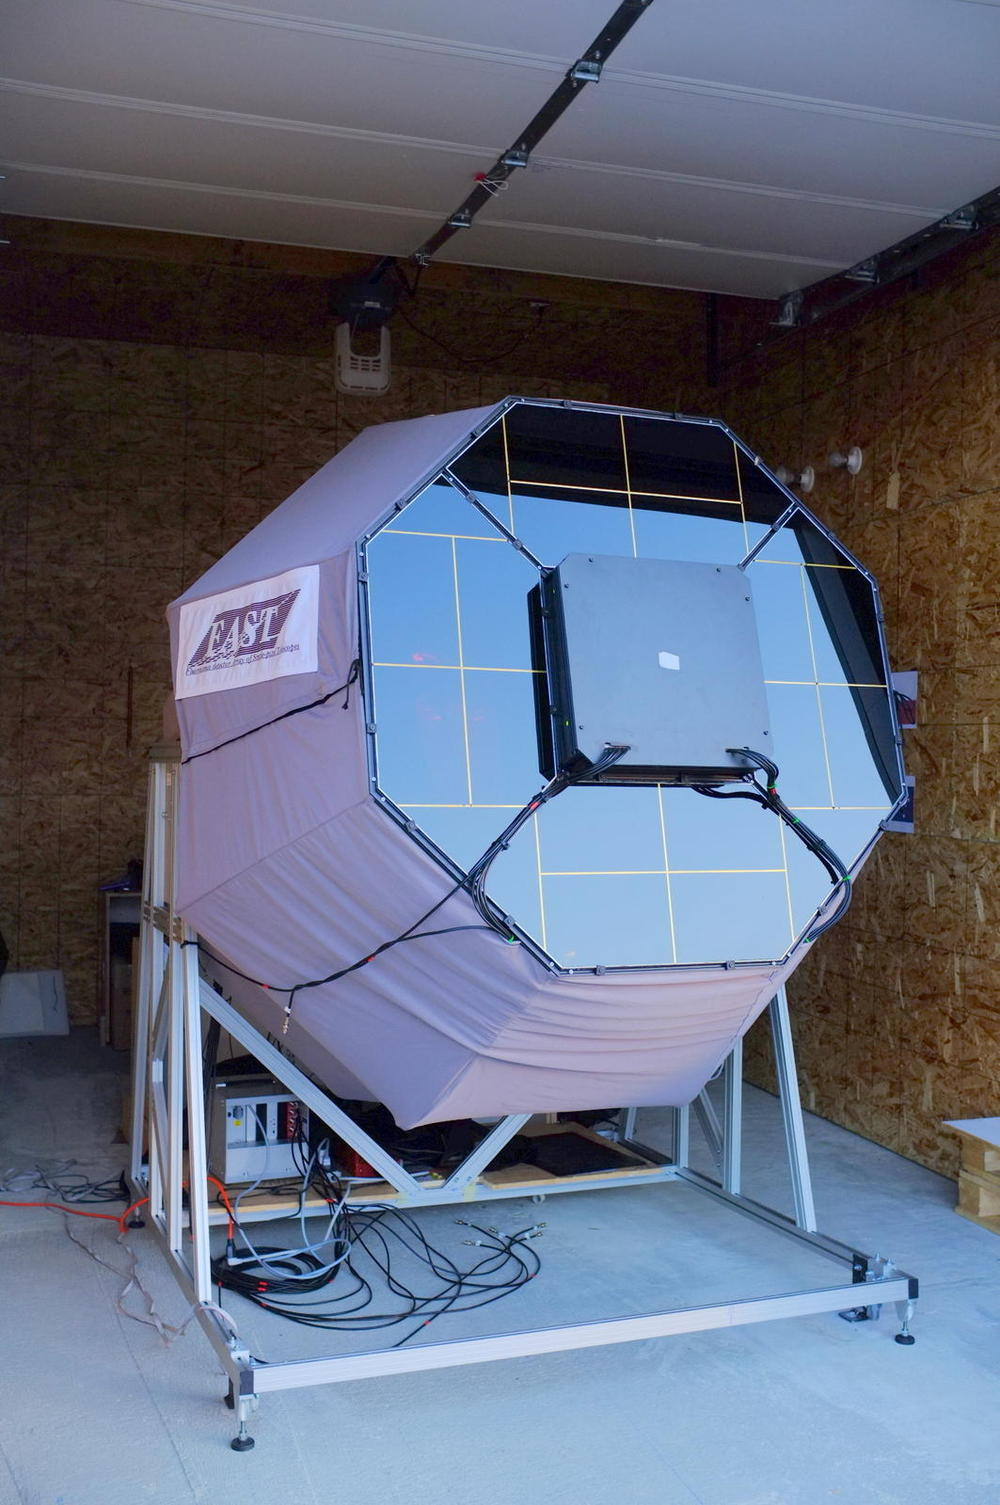
\includegraphics[scale = 0.15]{./pictures/FASTReal}}%
    \caption{FAST telescope.}%
    
     \label{FASThut}
\end{figure}


%\begin{figure}[H]
% \centering
% 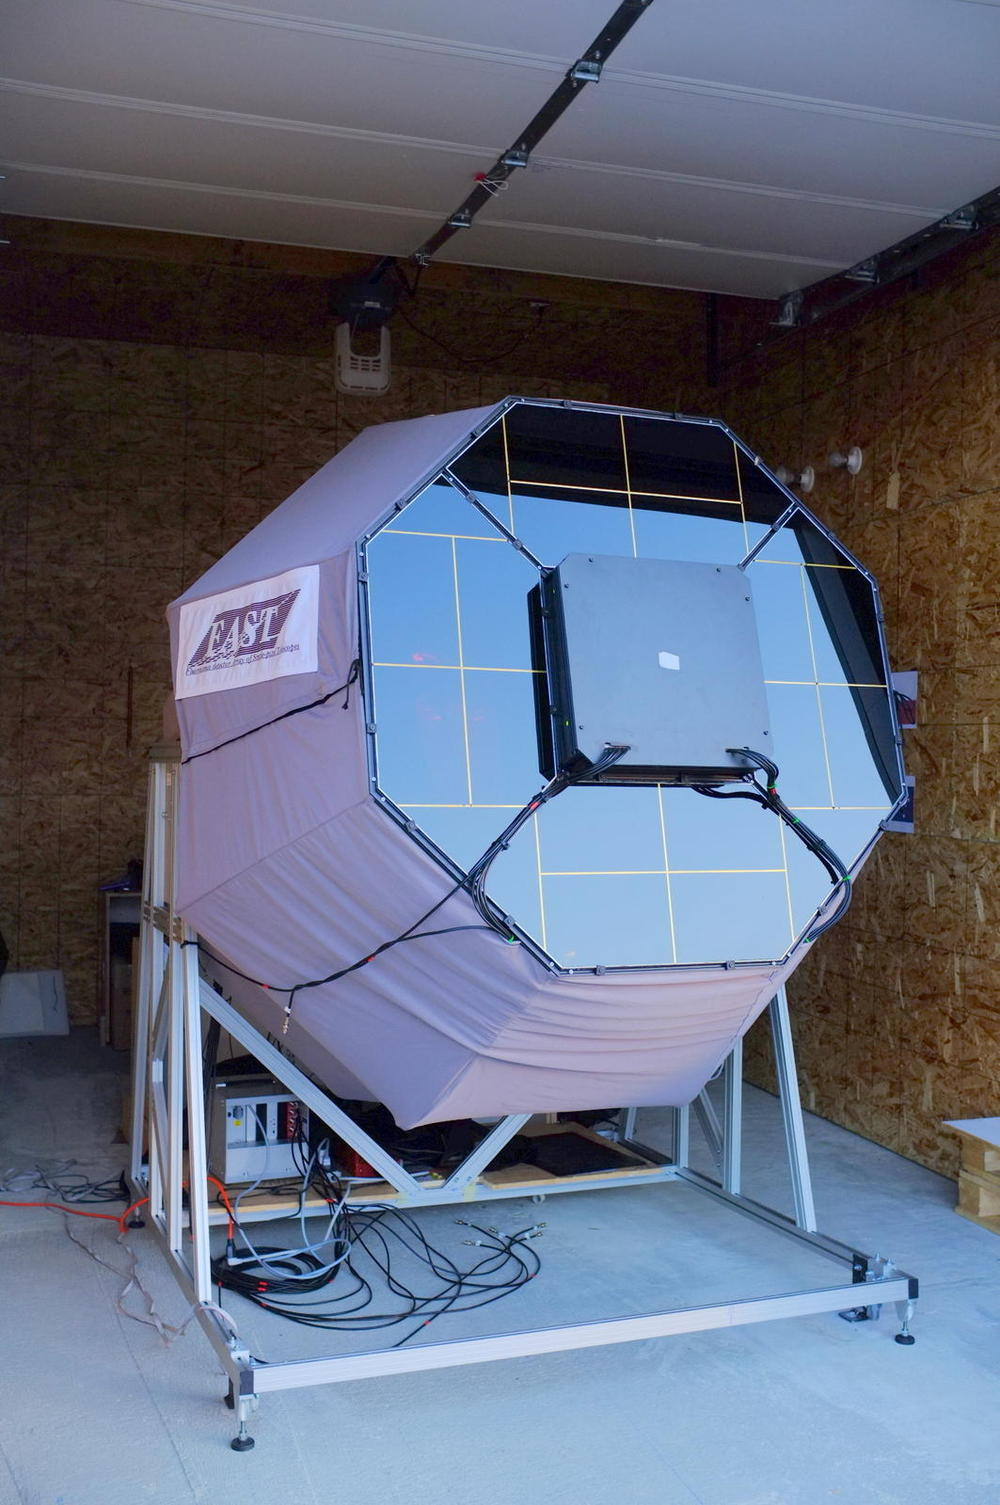
\includegraphics[scale = 0.2]{./pictures/FASTReal}
% \caption{FAST telescope \cite{Project}.}
% \label{FASThut}
 
%\end{figure}
% -----------------------------------------------
\section{FAST detection and operation scheme}
% -----------------------------------------------
Main detection part of the telescope consists of system of superreflective UV mirrors and 2x2 20cm PMT matrix (detection camera). The full specification of FAST optical concept could be found in \cite{Mandat_2017} and \cite{MALACARI2020102430}.

\par
%The optical design is similar to concept of lensless Schmidt camera\footnote{a catadioptric optical system consisting of lens and spherical mirror, which . The mirror This concept is excellent in providing large FoVs} - 

The current mirror system consists of primary circular mirror and 8 side mirrors (called petals), which focus the rays into detection camera. The camera is located 25~mm away from the focal plane further from the mirror to prevent the on-axis rays to focus in the dead space between PMTs. This concept gives FAST collecting area of 1~m$^2$ and a FoV (field-of-view) of $30^{\circ} \times 30^{\circ}$. On the fig. \ref{FASTConc} could be seen the simulation of the optical concept.



\begin{figure}[H]
 \centering
 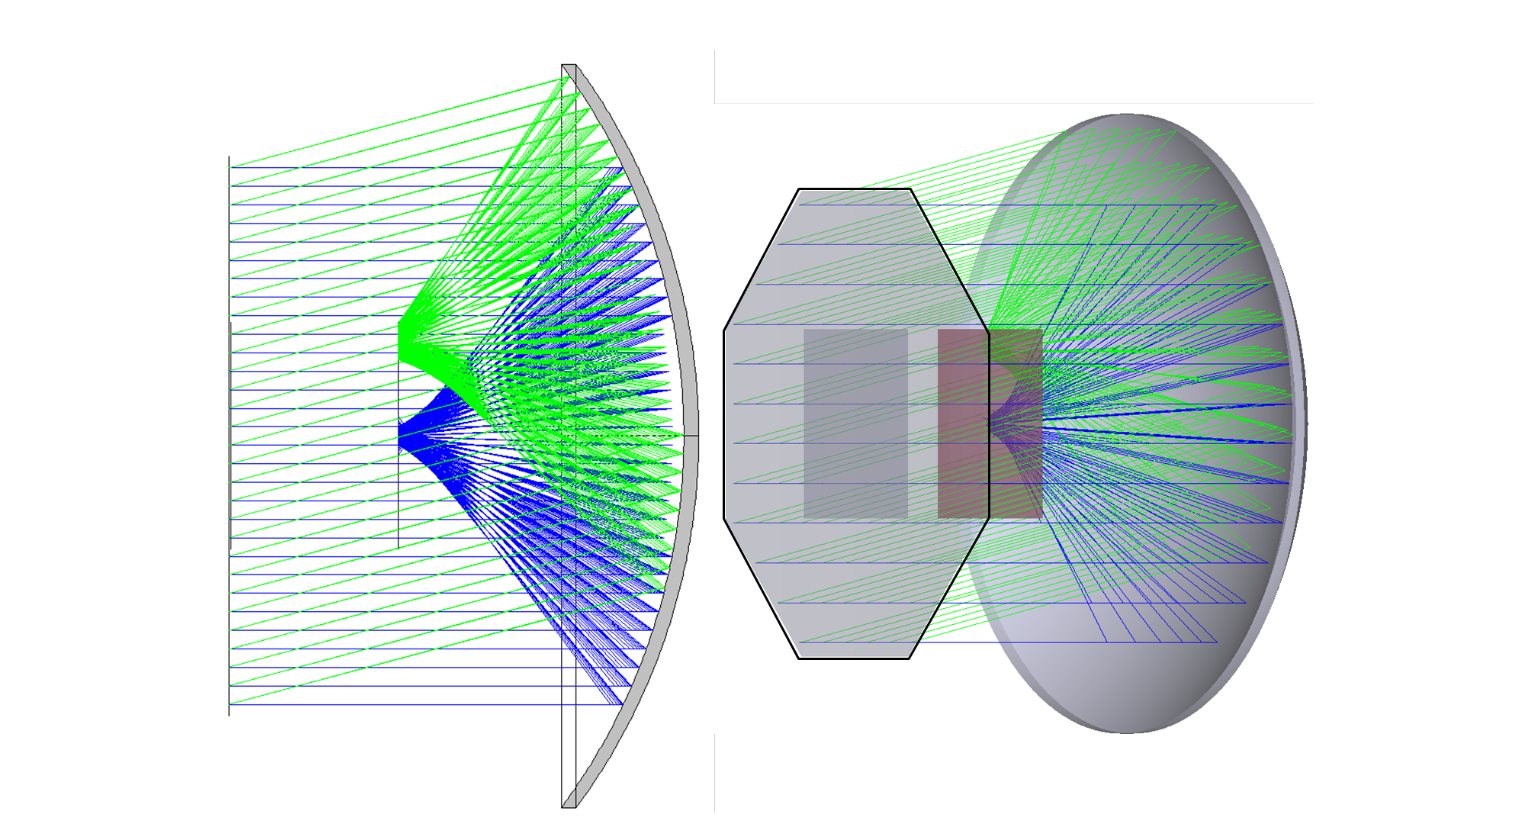
\includegraphics[scale = 0.2]{./pictures/FASTfocusing}
 \caption{Simulation of the FAST optical concept \cite{Mandat_2017}.}
 \label{FASTConc}
 
\end{figure}


\par
The aperture is covered by UV filter, which blocks the night-sky background photons ($\lambda > 400$ nm) and protects the mirrors.


\par
A NIM module provides a stable, low noise high voltage (900 - 1000 V) for all 4 PMTs, adjusting their gain around $10^5$. To establish same signal responsivity the different voltage can be adjusted to every single PMT.
\par
The data acquisition is handled by single-board PC, which runs the data acquisition software (DAQ). The DAQ controls the 14-bit FADC, which samples the pulses at rate 50 MSamples/s. The sampling can be triggered by internal high-threshold trigger or by external signal. Time stamps are provided by a GPS module. The raw data are stored in format containing signal waveforms, which can be later converted into the ROOT format, which we use in analysis.
\section{Protection hut}
Each telescope along with monitoring systems and other instruments is situated in a hut with remote controlled shutter, where it is protected from adverse phenomena, such as rain or fast wind, but also from dust and aerosols. Exposure of mirrors to any of this phenomena could lead to reduction of theirs reflectivity. It is also necessary to monitor and protect PMTs from unwanted light sources. Even a low-intensity sources could decrease PMT's service life.
% -----------------------------------------------

\section{Remote control and monitoring}
% -----------------------------------------------
In case of Argentina prototype, the telescope systems are connected to Pierre Auger network and through it, the telescope can be fully remote controlled and monitored over the internet. 

\par
Testing measurements, usually referred to as shifts, are performed in the night. Their main purpose is to acquire data, which can be later analysed and compared with data from Los Leones part of Pierre Auger, which has the similar FoV as Argentine FAST. 
The testing measurements require an operator to look after the telescope systems. An operator's duty is to power on and off the DAQ, PMTs' voltage sources, perform calibration, open and close the shutter and mainly check for failures and negative phenomena. To do that, operator can access webcam (\ref{FASTCam}), meteostation with thermometers, humidity, wind and light sensors and the All sky camera.

\par
This concept is similar to the Black Rock Mesa telescopes, but they are operated by Japanese.

\begin{figure}[H]
 \centering
 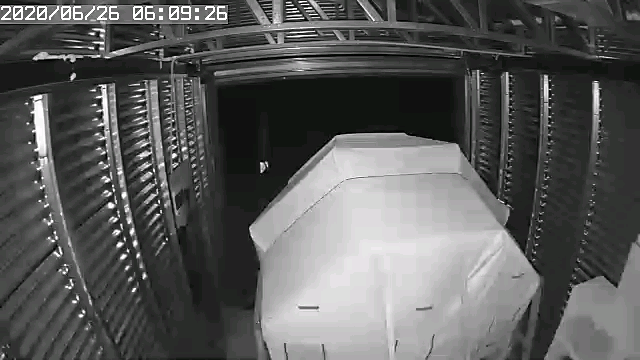
\includegraphics[scale = 0.5]{./pictures/operatinFast}
 \caption{FAST telescope with the open shutter from the webcam.}
 \label{FASTCam}
 
\end{figure}

%\begin{figure}[H]
% \centering
% 
\includegraphics{up_logo_bw}
% \caption{View from Allsky camera installed atop the hut. It gives the information %of sky quality by comparing visible stars with theoreretical star map.}
% \label{AllskyCam}
 
%\end{figure}







% -----------------------------------------------
% %%%%%%%%%%%%%%%%%%%%%%%% End of file %%%%%%%%%%%%%%%%%%%%%%%%
